\begin{center}
    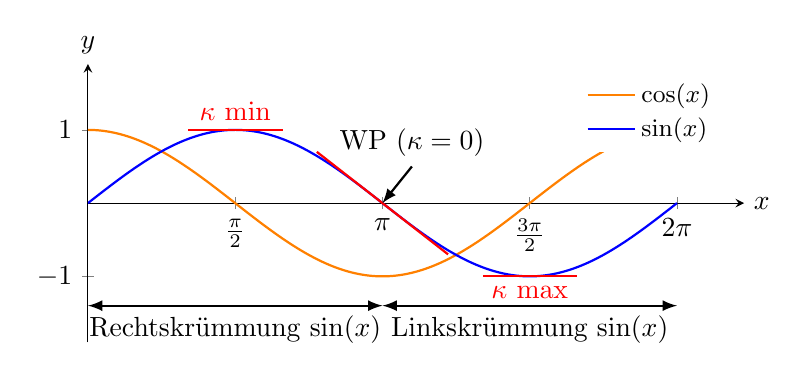
\begin{tikzpicture}
        \begin{axis}[
            scale=0.8,
            >=latex,
            xmin=0,
            xmax=7,
            ymin = -1.9,
            ymax = 1.9,
            width=12cm,
            height=6cm,
            samples=200,      
            axis x line=middle, 
            axis y line=middle, 
            xtick={0, pi/2, pi, 3*pi/2, 2*pi},
            xticklabels={$0$, $\frac{\pi}{2}$, $\pi$, $\frac{3\pi}{2}$, $2\pi$},
            ytick={-1, 0, 1},
            x label style={anchor=west},
            xlabel={$x$}, 
            y label style={anchor=south},
            ylabel={$y$},
            legend pos=north east,
            legend style={font=\small, cells={anchor=west}, draw=none}
        ]
        
        % cos()
        \addplot[orange, thick, domain=0:2*pi] {cos(deg(x))};
        \addlegendentry{$\cos(x)$}

        % sin()
        \addplot[blue, thick, domain=0:2*pi] {sin(deg(x))};
        \addlegendentry{$\sin(x)$}
        
        % Tangenten an sin()
        \addplot[red, thick, domain=pi/2-0.5:pi/2+0.5] {1};
        \node[above, red] at (pi/2, 1) {$\kappa$ min};

        \addplot[red, thick, domain=3*pi/2-0.5:3*pi/2+0.5] {-1};
        \node[below, red] at (3*pi/2, -1) {$\kappa$ max};

        \addplot[red, thick, domain=pi-0.7:pi+0.7] {-(x - 3*pi/2) - pi/2};

        \draw[->, thick] (1.1*pi, 0.5) node[above] {WP $(\kappa = 0)$} -- (pi, 0);

        \draw[<->, thick] (0, -1.4) -- (pi, -1.4) node[below, midway] {Rechtskrümmung $\sin(x)$};

        \draw[<->, thick] (pi, -1.4) -- (2*pi, -1.4) node[below, midway] {Linkskrümmung $\sin(x)$};

        \end{axis}
    \end{tikzpicture}
\end{center}

